\documentclass[12pt,letterpaper]{article}
%\usepackage{preamble}

%\ProvidesPackage{preamble}

\usepackage{fullpage}
\usepackage[top=2cm, bottom=4.5cm, left=2.5cm, right=2.5cm]{geometry}
\usepackage{amsmath,amsthm,amsfonts,amssymb,amscd}
\usepackage{lastpage}
\usepackage{enumerate}
\usepackage{fancyhdr}
\usepackage{mathrsfs}
\usepackage{xcolor}
\usepackage{graphicx}
\usepackage{listings}
\usepackage{hyperref}
\usepackage{enumitem}
\usepackage{float}
\usepackage{fancyvrb}
\usepackage{color,soul}
\sethlcolor{lightgray}
 \usepackage{subfigure}
 \usepackage{textcomp}
\usepackage{siunitx}

\usepackage{graphicx}
\usepackage{array}

\usepackage[T1]{fontenc}
\usepackage[numbered,framed]{matlab-prettifier}
\hypersetup{%
  colorlinks=true,
  linkcolor=blue,
  linkbordercolor={0 0 1}
}

\let\ph\mlplaceholder % shorter macro
\lstMakeShortInline"

\lstset{
  style              = Matlab-editor,
  basicstyle         = \mlttfamily \small,
  escapechar         = ",
  mlshowsectionrules = true,
  xleftmargin=.01\textwidth, xrightmargin=.01\textwidth
}

\graphicspath{{./problem1_images}}

\pagestyle{fancyplain}
\headheight 35pt
\lhead{\userID}
\chead{\textbf{\Large Project \hwnumber}}
\rhead{\course \\ \today}
\lfoot{}
\cfoot{}
\rfoot{\small\thepage}
\headsep 1.5em




%%%%%%%%%%%%%%%%%%%%%%%%%%%%%%%%%%%%%%%%%%
%%%% Edit These for yourself
%%%%%%%%%%%%%%%%%%%%%%%%%%%%%%%%%%%%%%%%%%
\newcommand\course{Econ 672}
\newcommand\hwnumber{1}
\newcommand\userID{Ziming Huang}
\newenvironment{alphaparts}[0]{%
  \begin{enumerate}[label=\textbf{\Alph*}]
}{\end{enumerate}}


\begin{document}
%\textbf{\Large PROJECT 1}



 




\section*{Exercise 1}
  \begin{enumerate}[label=\textbf{(\Alph*)}]
%----A-----
  \item Interprets of parameters:\\
 	 	  \emph{n}: The number of steps per unit time;\\
 	      \emph{T}: The total observe time;\\
 	      \emph{$\mu$}: The risk premium (mean) of holding asset during a time unit (day);\\
 	      \emph{$\sigma$}: The standard deviation of asset price during a time unit (day).\\
 	      
 	      Assuming the trading time for a year is T, then we have: \begin{center}
 	      	\begin{align}
 	      	 E(X_T^n)&=T*E(X_1^n)=T\mu \\
 	      	 sd(X_T^n)&=\sqrt{Var(X_T^n)}=\sqrt{T*Var(X_1^n)}=\sqrt{T}\sigma
 	      	\end{align}
 	      \end{center}	    
 %----B-----
 \item In order to stimulate the continuous time process of asset price P, we need to decompose the continuous time into small time interval (step):
 
 	 \begin{center}
 	 	\begin{align}
 	 X_i=X_{i-1}+\mu\Delta_n+\sigma\sqrt{\Delta_n}Z_i
 	 \end{align}
     \end{center}  

\mbox{then we have:}
    \begin{center}
  	   \begin{align}
    X_i-X_{i-1}&=\mu\Delta_n+\sigma\sqrt{\Delta_n}Z_i \\
    X_n^T&=\sum_{i=1}^{\emph{nT}/\Delta_n}{(\mu\Delta_n+\sigma\sqrt{\Delta_n}Z_i)}
    	\end{align}
    \end{center}  
  Here ${Z_i}$ are identical independent normal distribution, that is ${Z_i} \sim  \mathcal{N}(0,1)$ for \emph{i} = 1,2 $\cdots$, nT.\\
  
  To construct $X_n^T$:
  \begin{enumerate}[label=(\roman*)]
  	\item Construct a series number from the standard normal distribution;
  	\item Adding each component in equation(5);
  	\item Converting the log-price to prices.
  \end{enumerate}
 
  Here is the plot of time series prices:
        \begin{figure}[H]
            \centering
            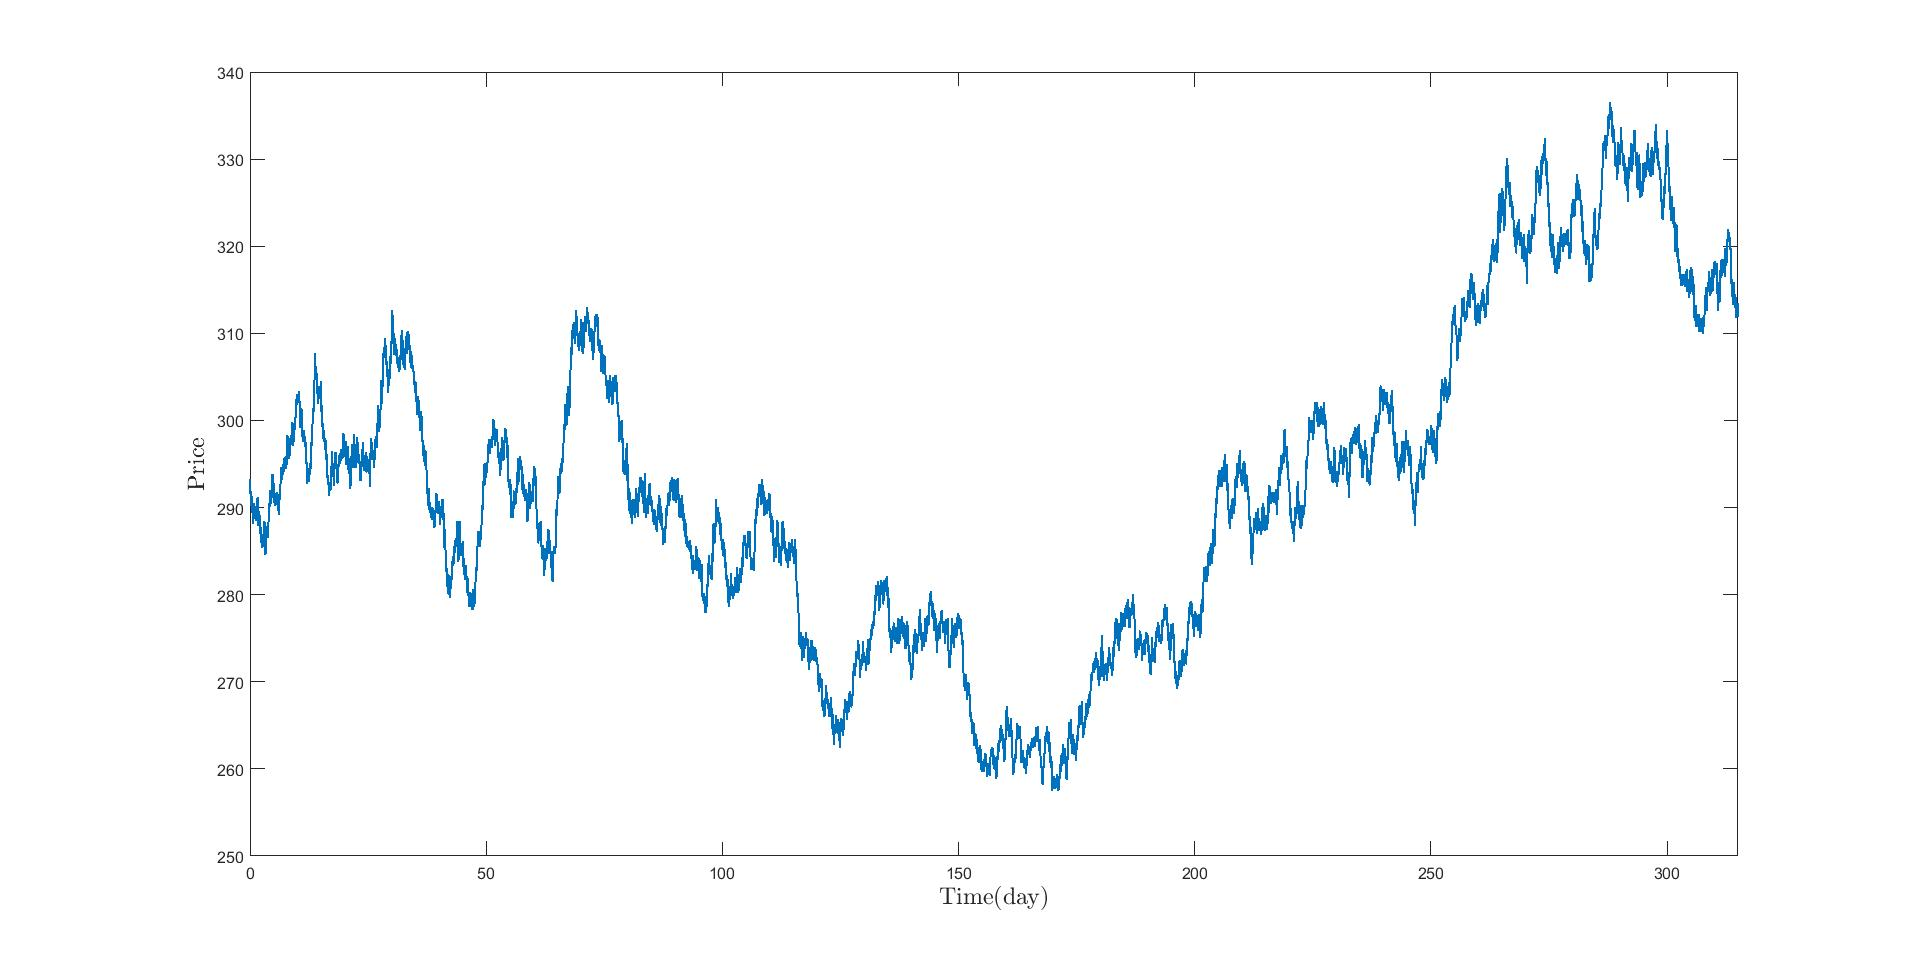
\includegraphics[width=15cm]{figures/p1_ex1.jpg}
            \caption{Time Series Prices (Gaussian Diffusion with Constant Coefficients)}
            \label{fig:1}
        \end{figure}
 From the figure, we can see the price range is (200,340) and the price fluctuates a lot.\\
 
  The \textbf{MATLAB} code:
   \lstinputlisting{functions/GD_c.m}
   
   \lstinputlisting{scripts/p1_ex1.m}
\end{enumerate}
\newpage

%---------------------------------------------


\section*{Exercise 2}
  \begin{enumerate}[label=\textbf{(\Alph*)}]
%----A-----
  \item Interprets of parameters:\\
 	      \emph{$\lambda$}: The density of Poisson distribution during a time unit(per day);\\
 	      \emph{$\sigma_j$}: The standard deviation of step jump.\\
 	      \\
 	      Here $\sigma$ is the standard deviation of daily jump, while $\sigma_j$ is the standard variance of jump of every step. Since every day is divided into \emph{n} steps, we need to convert daily standard deviation to step standard deviation by divided $\sqrt{n}$.
%----B-----
  \item To construct compound Poisson process $J_i$:
      \begin{enumerate}[label=(\roman*)]
  	    \item Produce a Poisson distribution with density $\lambda$T to product the jump number \emph{N};
  	    \item Produce jump time by producing \emph{N} random number from Unif $\sim (0,T)$;
      	\item Produce jump size by producing \emph{N} random number from $\mathcal{N}(0,1)$;
      \end{enumerate}
 
Here is the plot of time series prices:
        \begin{figure}[H]
            \centering
            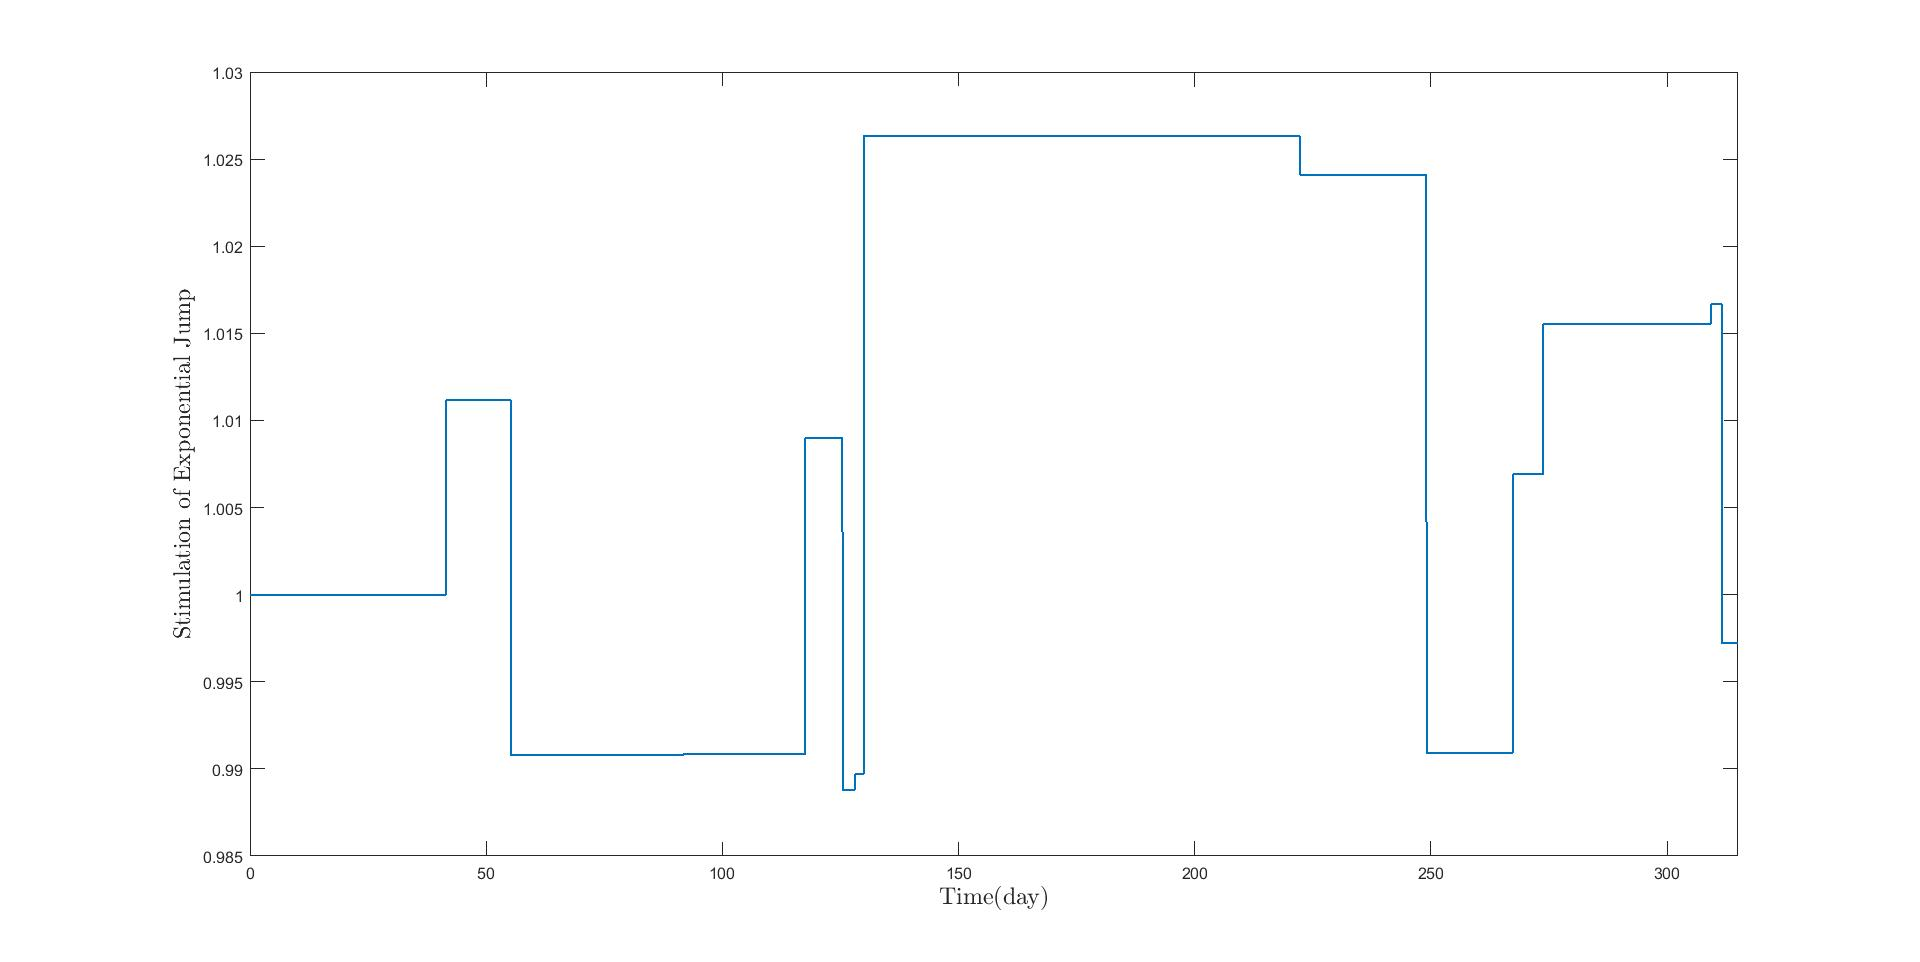
\includegraphics[width=15cm]{figures/p1_ex2.jpg}
            \caption{Time Series of Exponential Jump}
            \label{fig:2}
        \end{figure}
From the figure, we can see there are total 12 times of jump during our observation (from time=0 to 315). The (exponential) jump size range from 0.85 to 1.03. Among these 12 jumps, 7 of them are upside jumps, while 5 of them are downside jumps.\\
 
  The \textbf{MATLAB} code:
  \lstinputlisting{functions/jump.m}
  
  \lstinputlisting{scripts/p1_ex2.m}
\end{enumerate}
\newpage

%---------------------------------------------
\section*{Exercise 3}
  \begin{enumerate}[label=\textbf{(\Alph*)}]
%----A-----
  \item Both expression 1 and 4 are correct. Expression 1 is the log-price (with log-jump) of asset, while expression 4 is the price (with jump) of asset.
 	      
%----B-----
\item  Here use expression 4 to calculate the price (with jump) of asset.Following is the plot of time series prices:
        \begin{figure}[H]
            \centering
            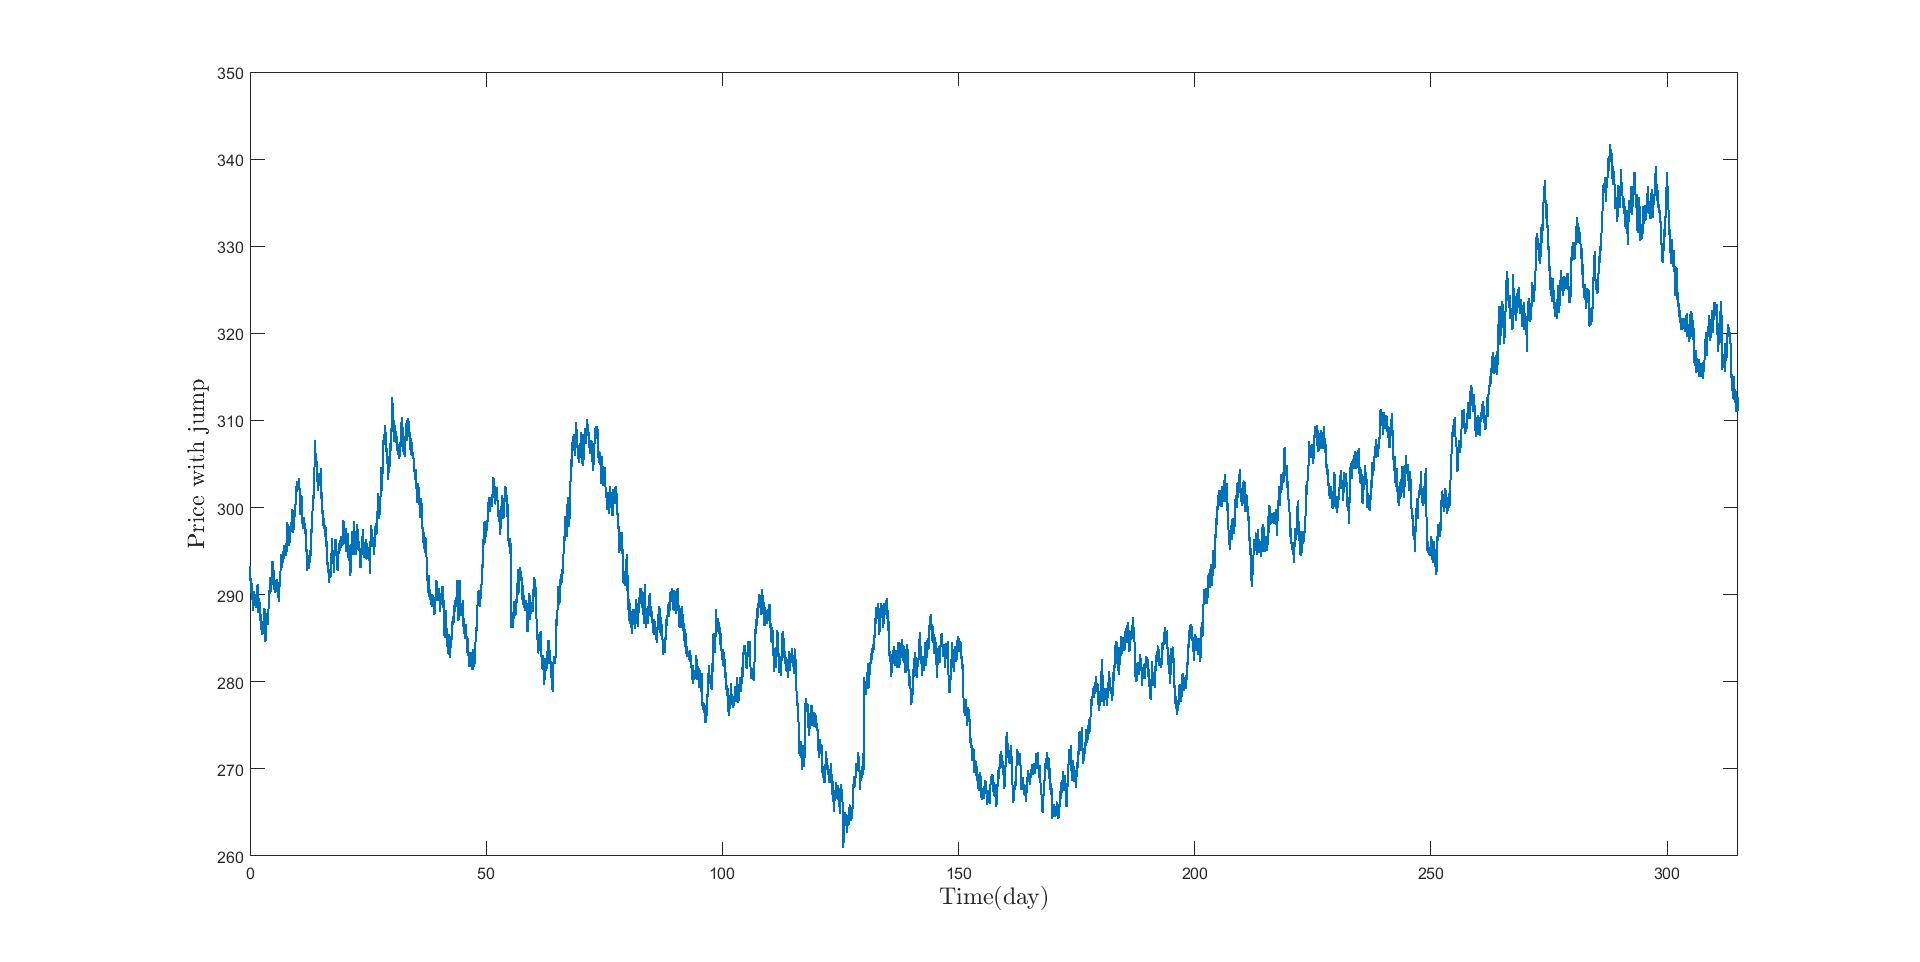
\includegraphics[width=15cm]{figures/p1_ex3.jpg}
            \caption{Time Series of Price with Jump}
            \label{fig:3}
        \end{figure}
Compare to figure in Exercise 1, we can see the price range doesn't change a lot, but the fluctuation of price has increased.\\

The \textbf{MATLAB} code:
   \lstinputlisting{scripts/p1_ex3.m}
   %\newpage
\end{enumerate}
\newpage
%---------------------------------------------




\section*{Exercise 4}
  \begin{enumerate}[label=\textbf{(\Alph*)}]
%----A-----
  \item Interprets of parameters:\\
 	      \emph{$\rho$}: The rate of convergence;\\
 	      \emph{$\mu_c$}: The mean of step price volatility.\\
 	      \emph{$\sigma_c$}: The volatility of step price volatility.
%----B-----$
\item  To construct stochastic variance process $c_j$:
  \begin{enumerate}[label=(\roman*)]
  	\item Construct a series number from the standard normal distribution;
  	\item Compute each ${c_j}$ by iteration;
  \end{enumerate}
 
Here is the plot of time series prices:
        \begin{figure}[H]
            \centering
            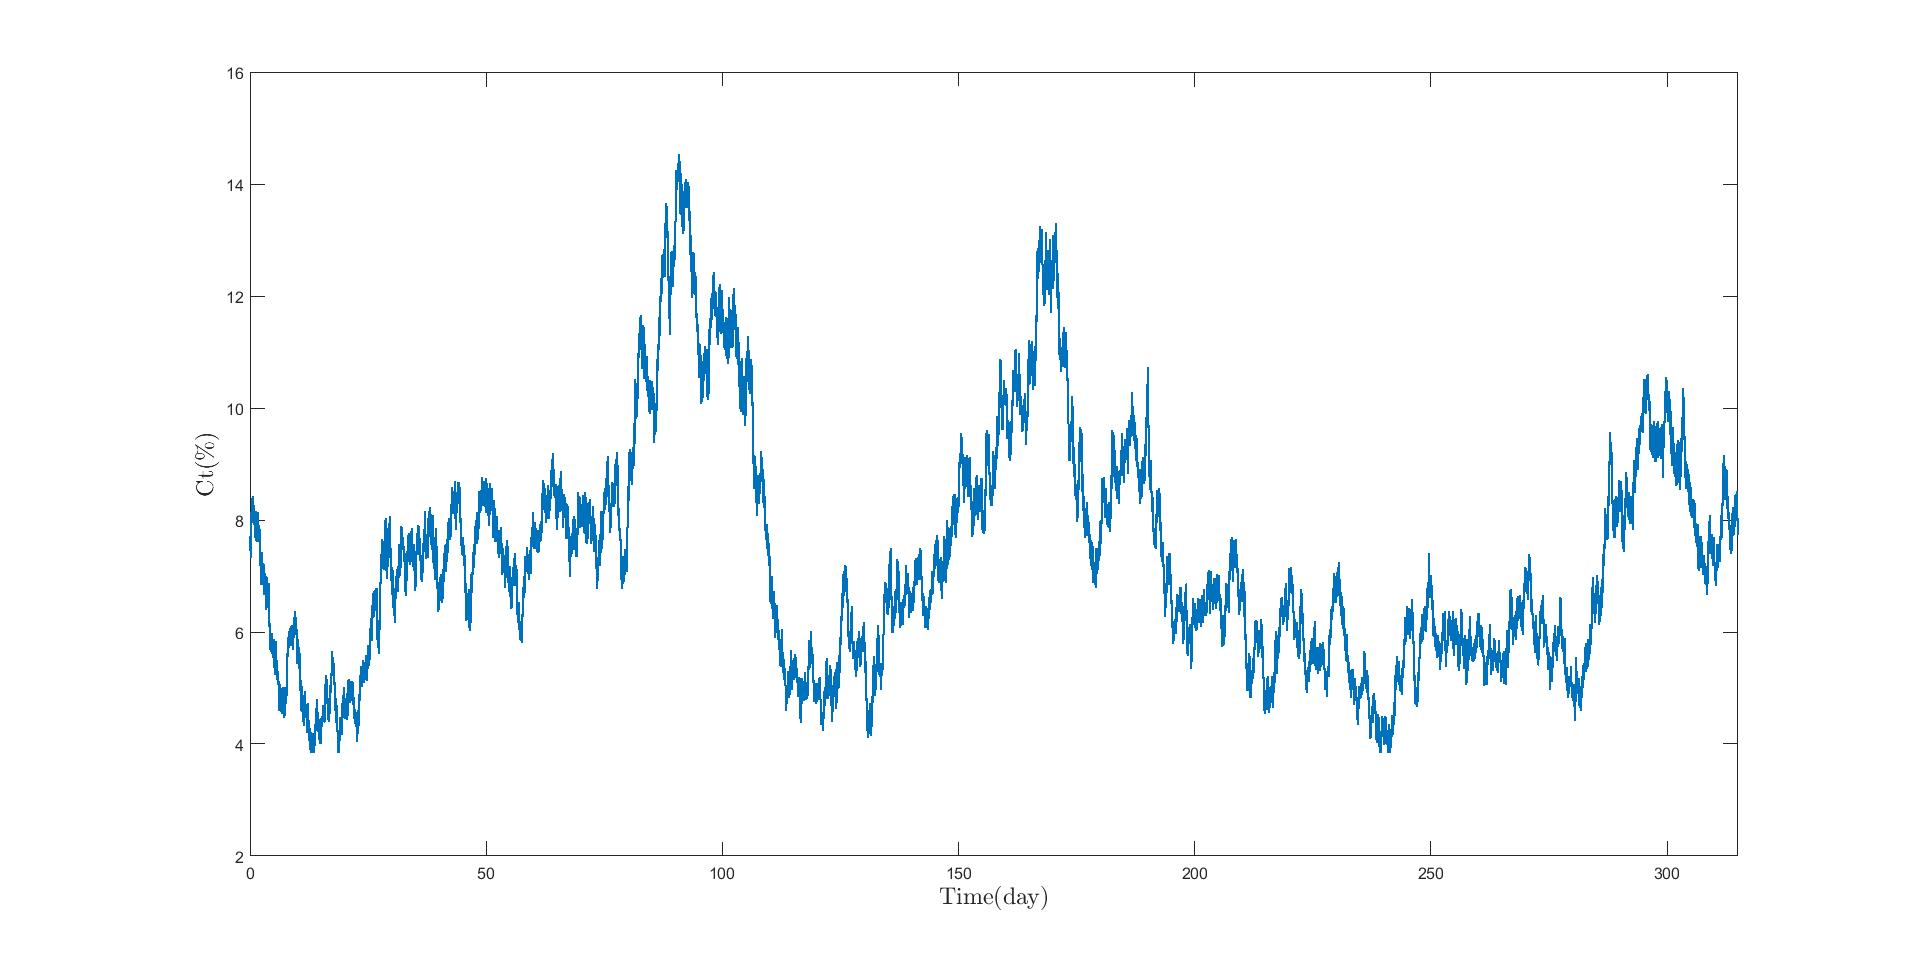
\includegraphics[width=15cm]{figures/p1_ex4_b.jpg}
            \caption{Stimulation of Annual Ct}
            \label{fig:4b}
        \end{figure}
From the figure, we can see at time around 40, 100, 180 and 300, there are large jump of Ct.
%----c-----
\item  To construct high frequency log-price $X_j$:
  \begin{enumerate}[label=(\roman*)]
  	\item Construct a series number from the standard normal distribution;
  	\item Use ${c_j}$ to compute each ${X_j}$ by iteration;
  \end{enumerate}
Here is the plot of time series prices:
        \begin{figure}[H]
            \centering
            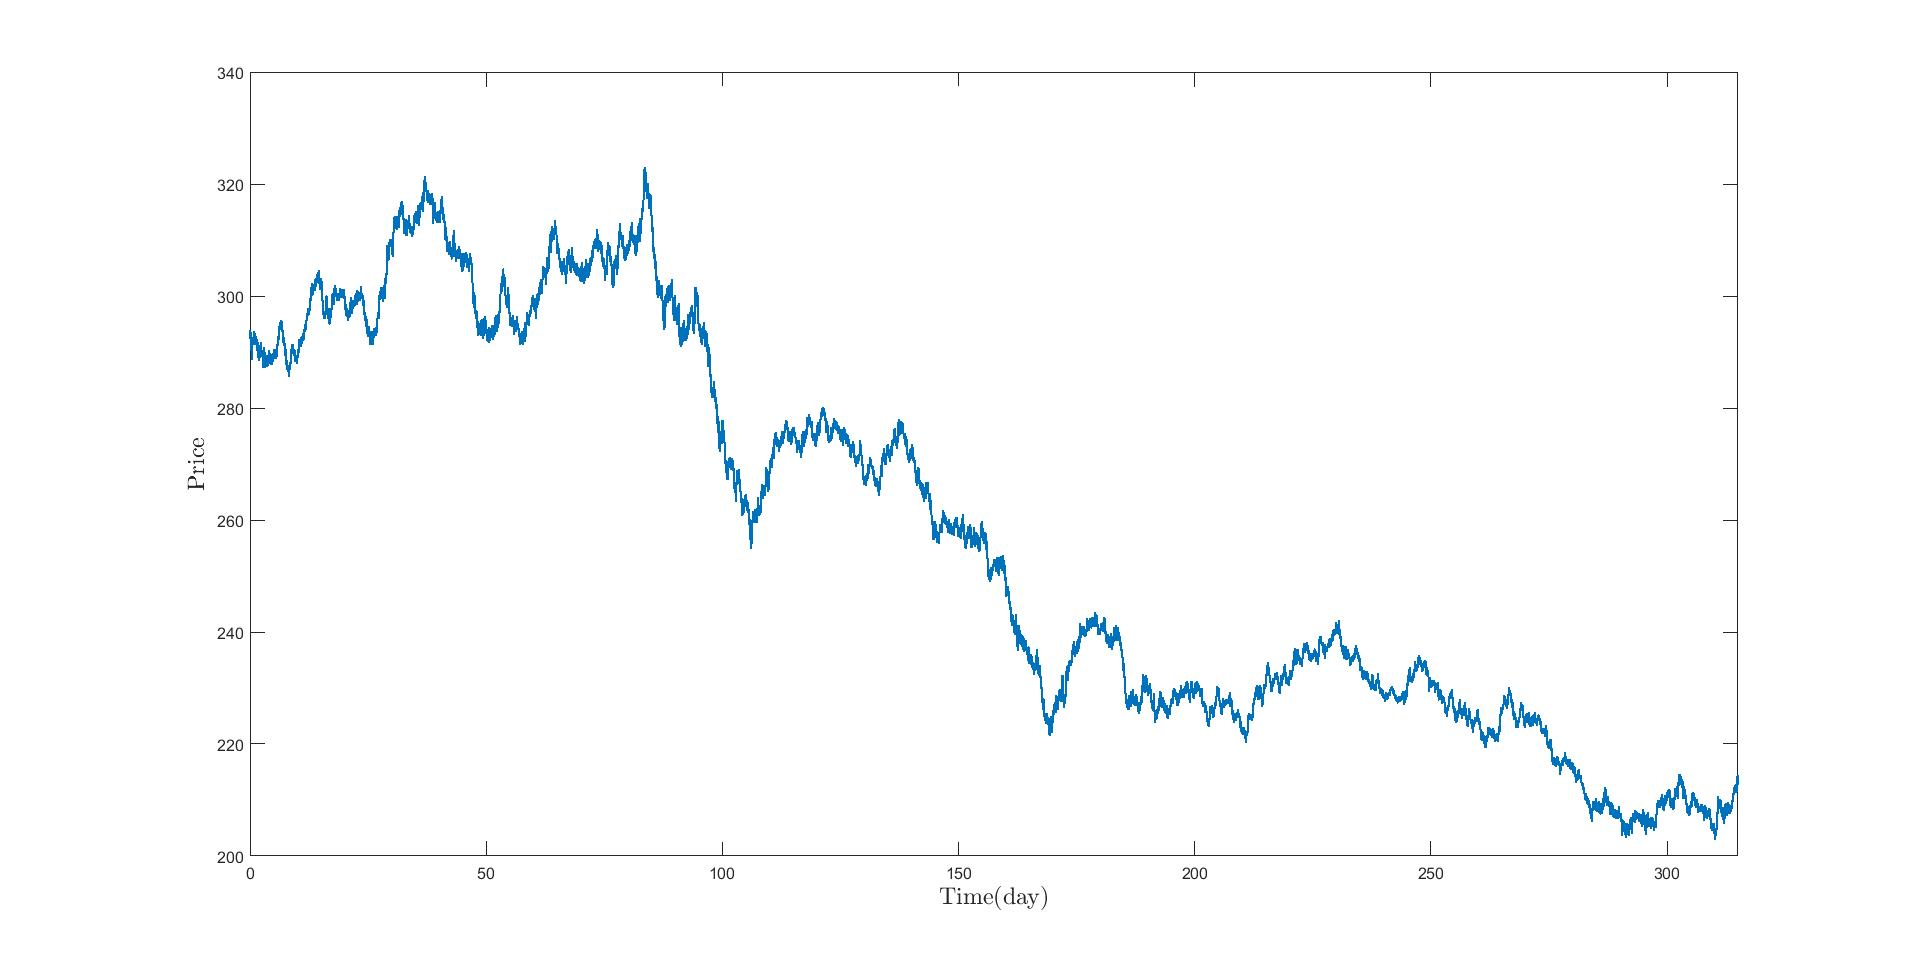
\includegraphics[width=15cm]{figures/p1_ex4_c.jpg}
            \caption{Stimulated of Time Series Price Xt (Use High Frequency Samples}
            \label{fig:4c}
        \end{figure}     
From the figure, those we can see at time around 40, 100 and 180 and 300, Xt has large jump, too.
        
        
%----d-----
\item Here is the plot of time series log-return:
        \begin{figure}[H]
            \centering
            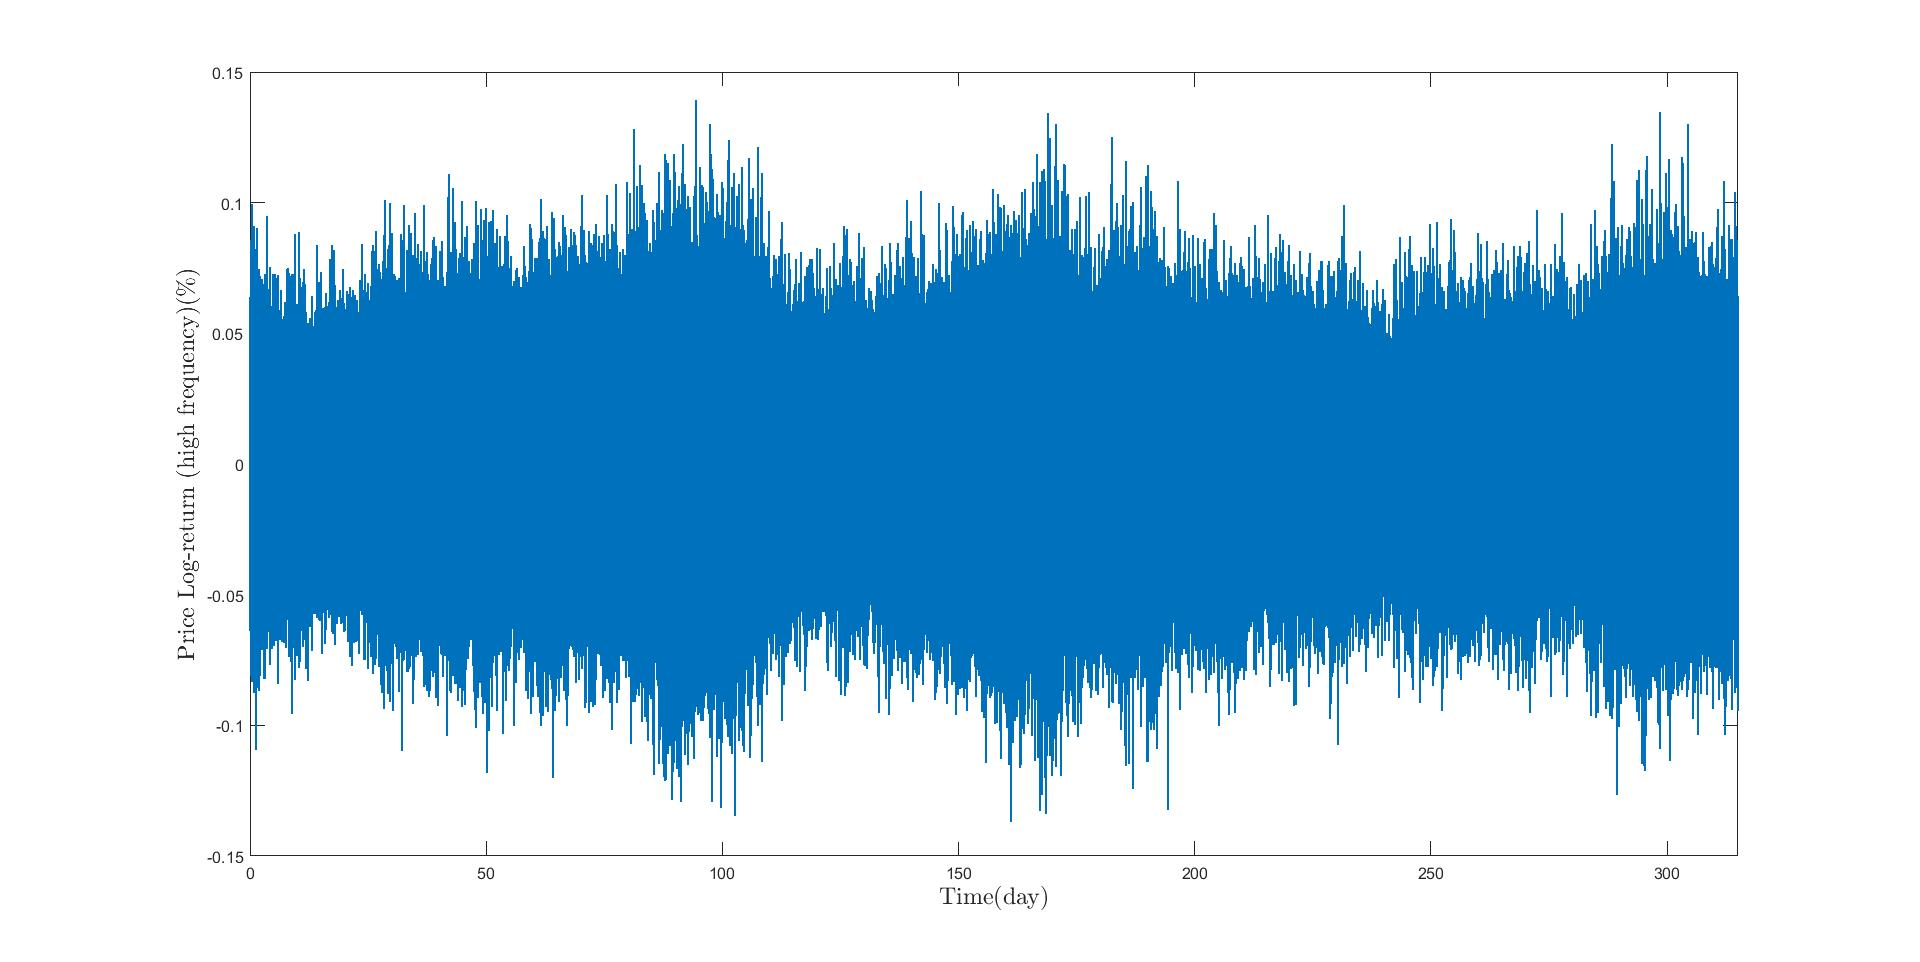
\includegraphics[width=15cm]{figures/p1_ex4_d.jpg}
            \caption{Time Series Log-return (Use High Frequency Samples)}
            \label{fig:4d}
       \end{figure} 
From the figure, those we can see at time around 40, 100 and 180 and 300, where Xt has large jump, the price log-return fluctuates a lot , so well as the log-return in their neighbor time interval.We can find the pattern of volatility clustering.       
%----e-----
\item Here is the plot of time series log-return with coarser frequency sample:
        \begin{figure}[H]
            \centering
            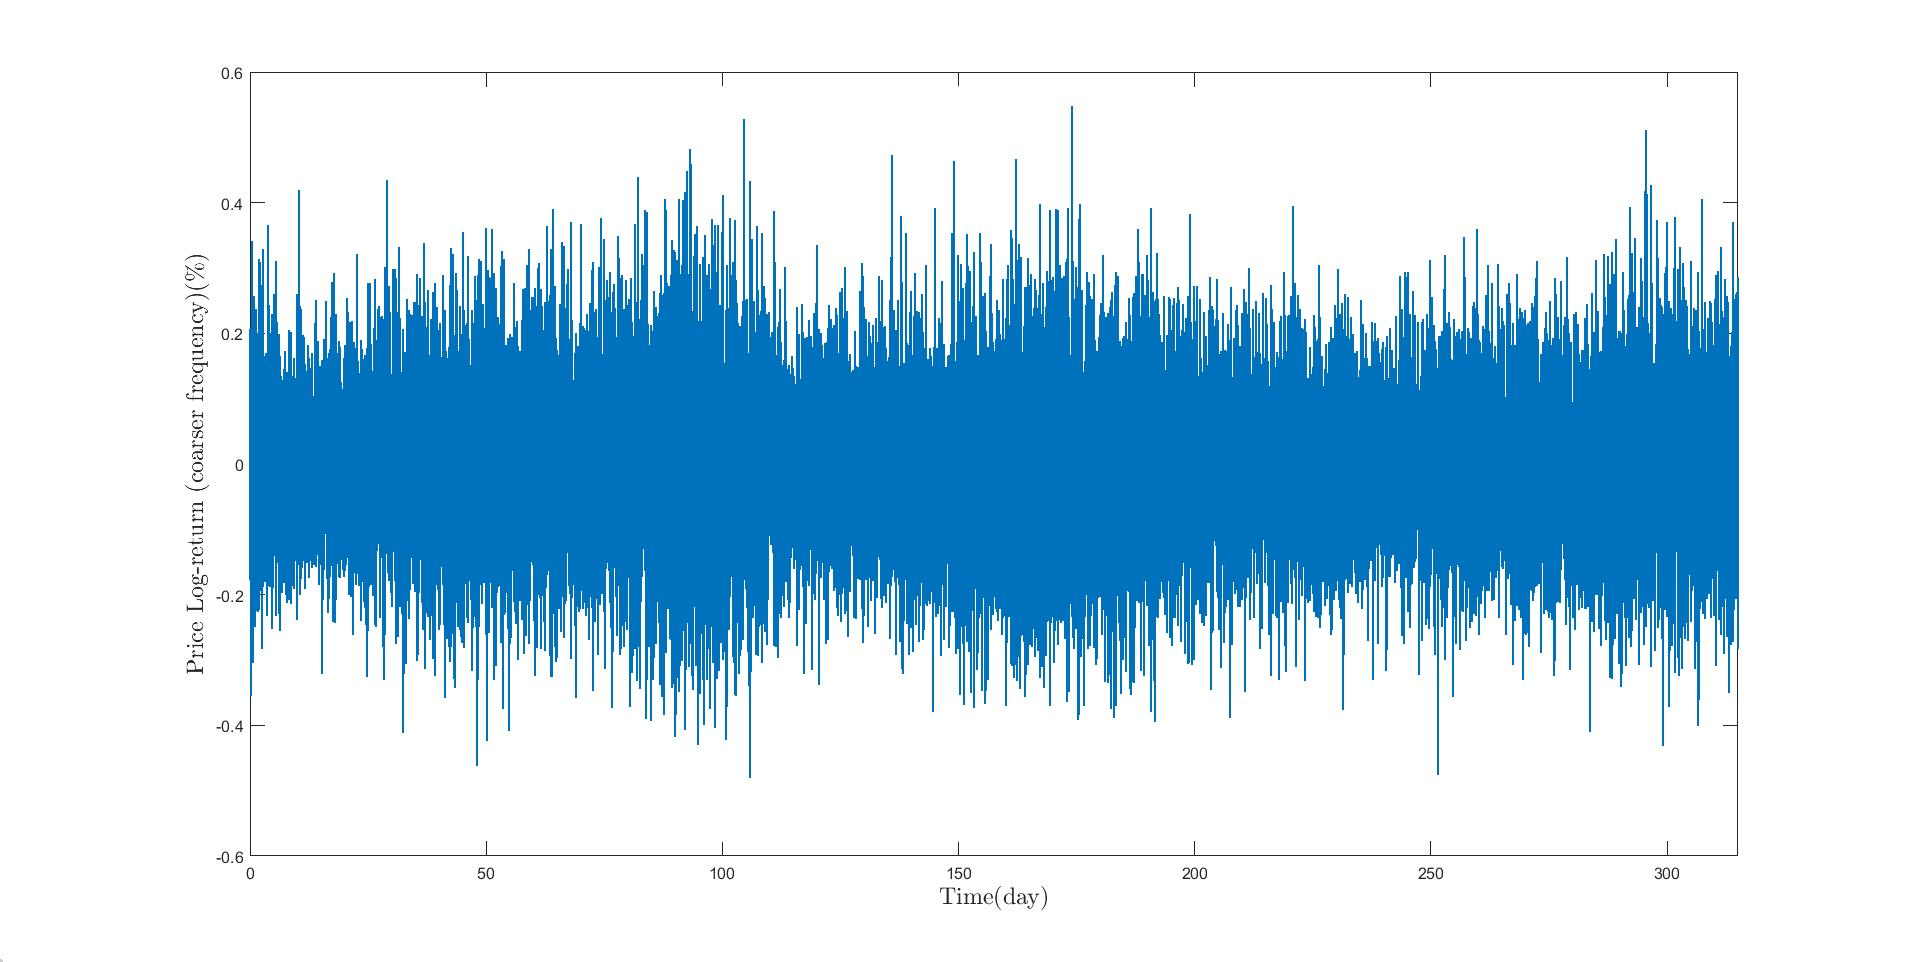
\includegraphics[width=15cm]{figures/p1_ex4_e.jpg}
            \caption{Time Series Log-return (Use Coarser Frequency Samples)}
            \label{fig:4e}
        \end{figure}    
From the figure we can find the pattern of volatility clustering is more obvious than the case using high frequency sample.
%----f-----
\item Here are the plots of stochastic volatility with different rate of convergence $\rho$:
        \begin{figure}[H]
            \centering
            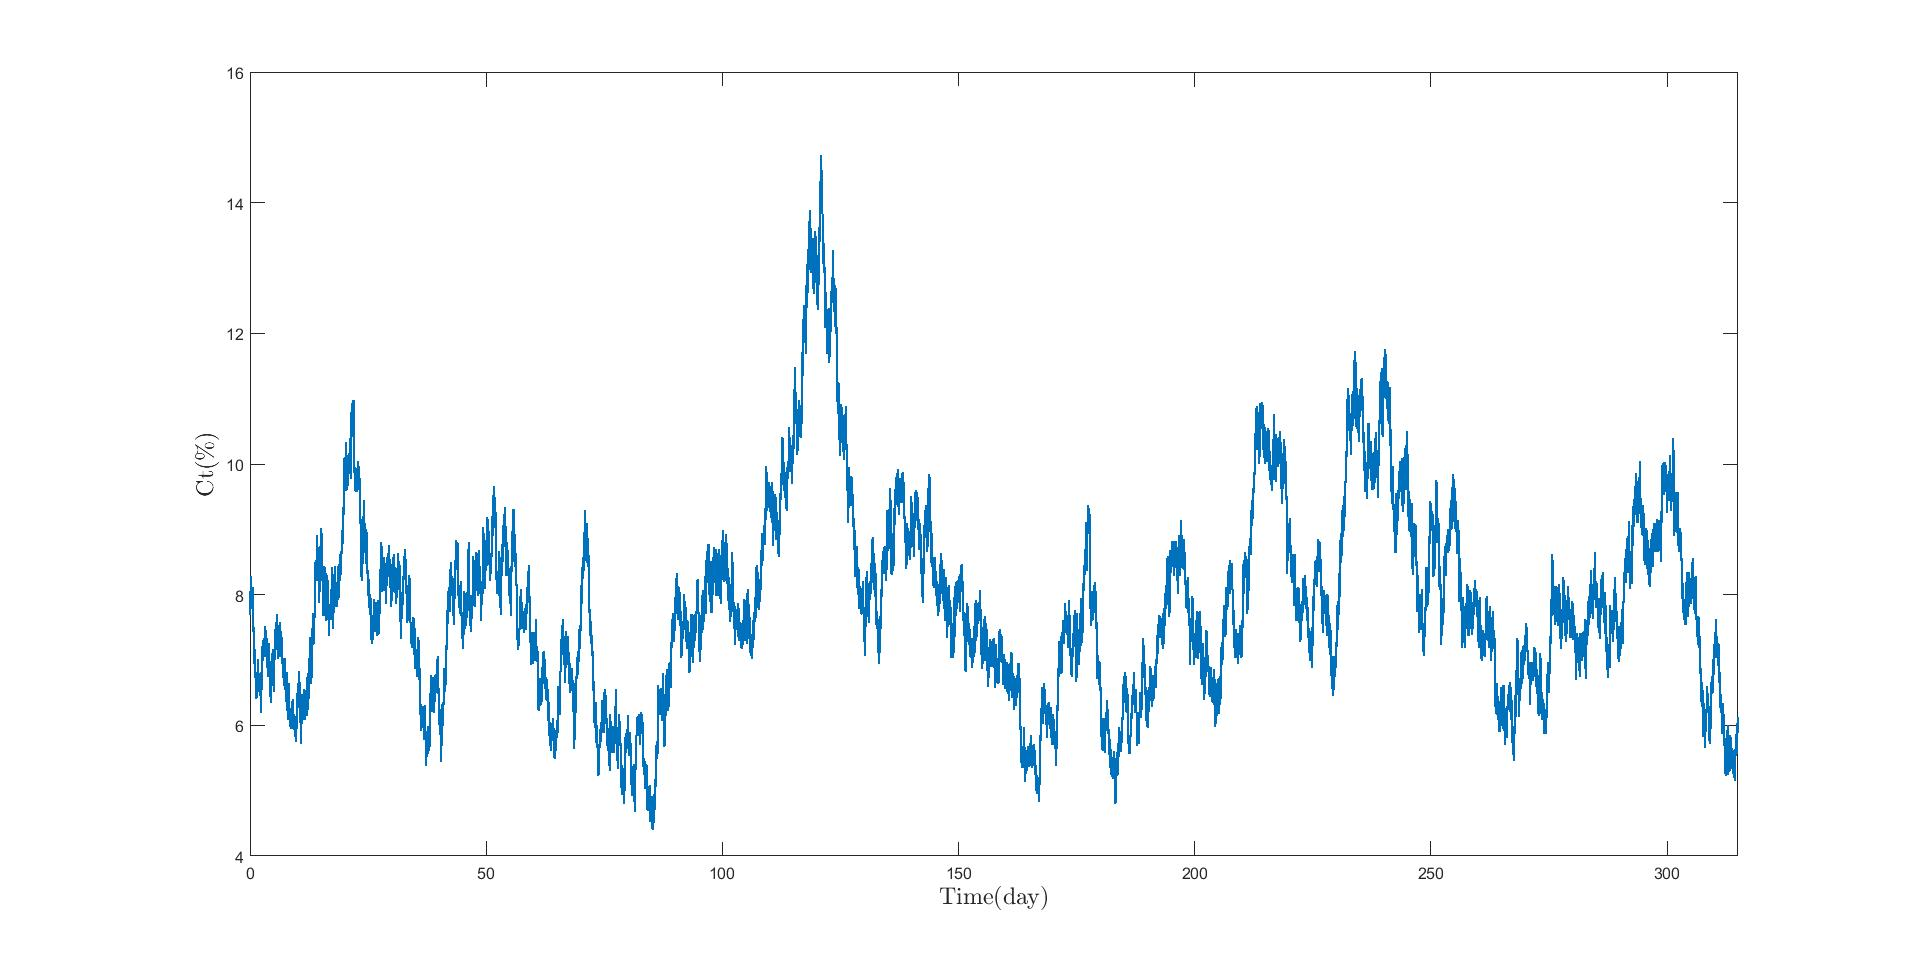
\includegraphics[width=15cm]{figures/p1_ex4_f1.jpg}
            \caption{Stochastic Volatility Ct with $\rho=0.03$}
            \label{fig:4_f1}
            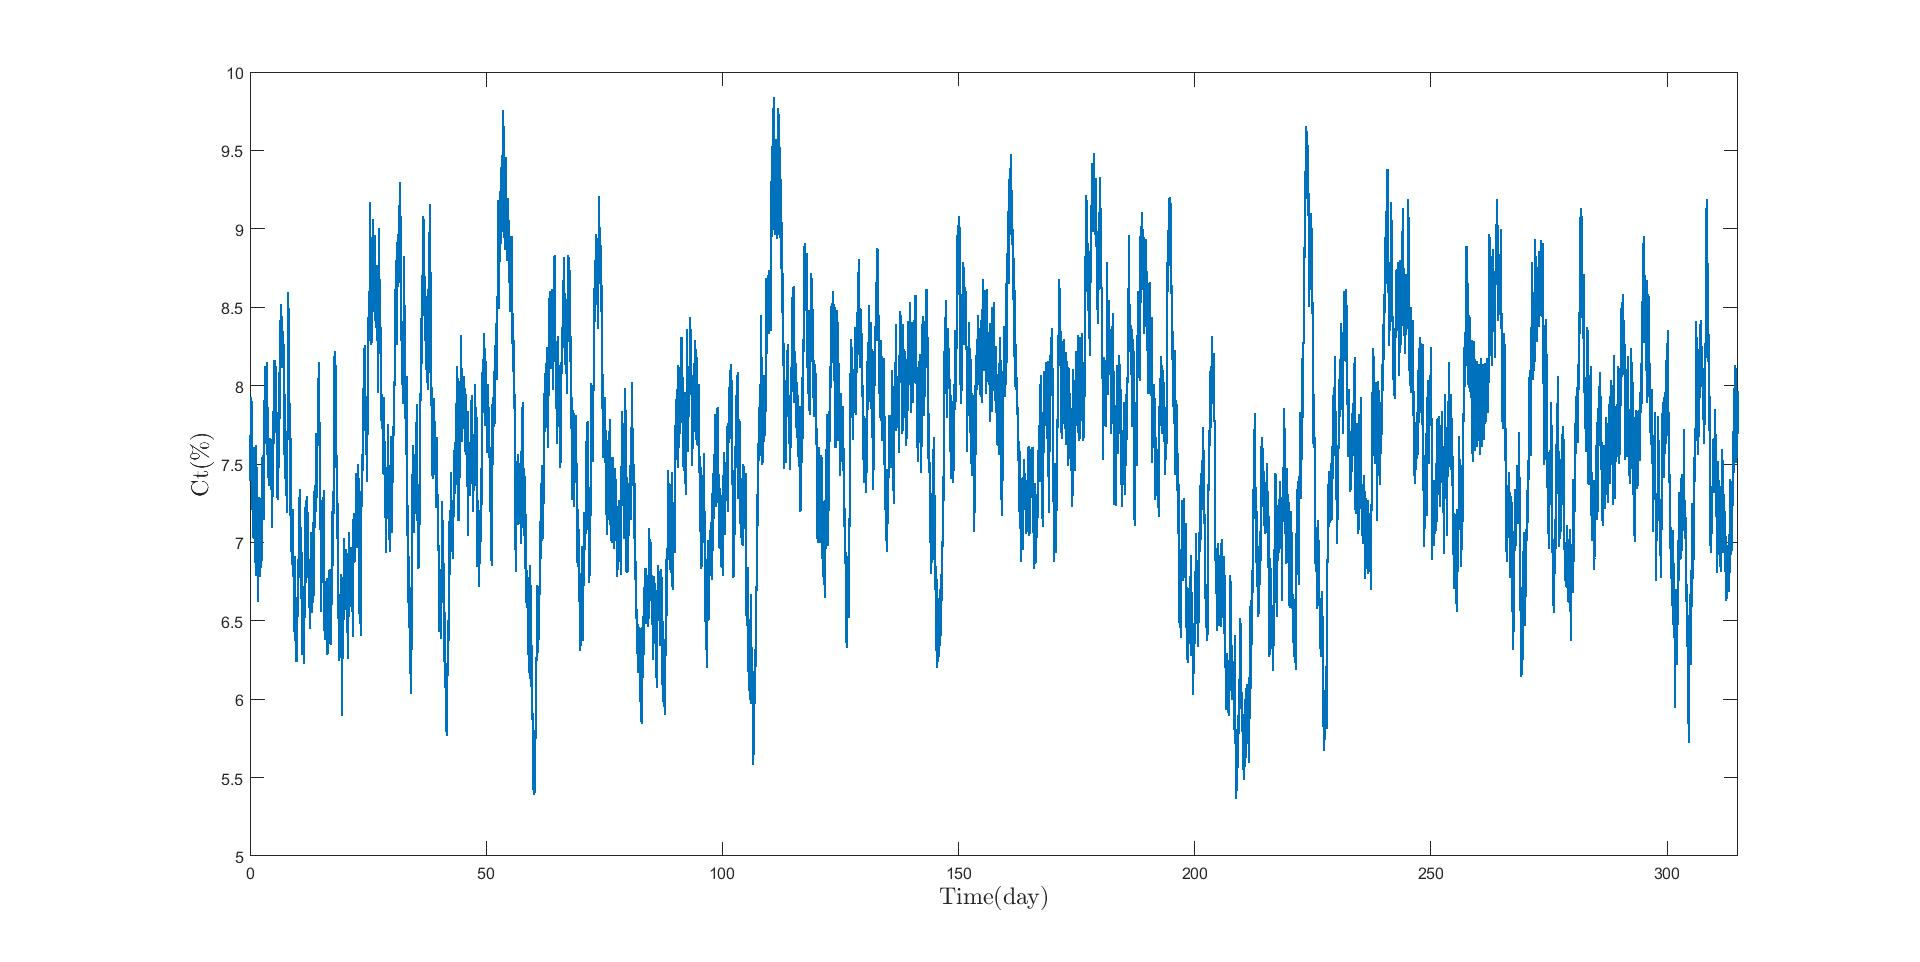
\includegraphics[width=15cm]{figures/p1_ex4_f2.jpg}
            \caption{Stochastic Volatility Ct with $\rho=0.1$}
            \label{fig:4_f2}
        \end{figure}
From the figure, we can find as the rate of convergence $\rho$ increases, the pattern that price stochastic volatility Ct fluctuates around its mean becomes more obvious, that is, the price stochastic volatility Ct converges at a faster speed.
%----g-----
\item Here are the plots of stochastic volatility with different volatility $\sigma_c$:
        \begin{figure}[H]
            \centering
            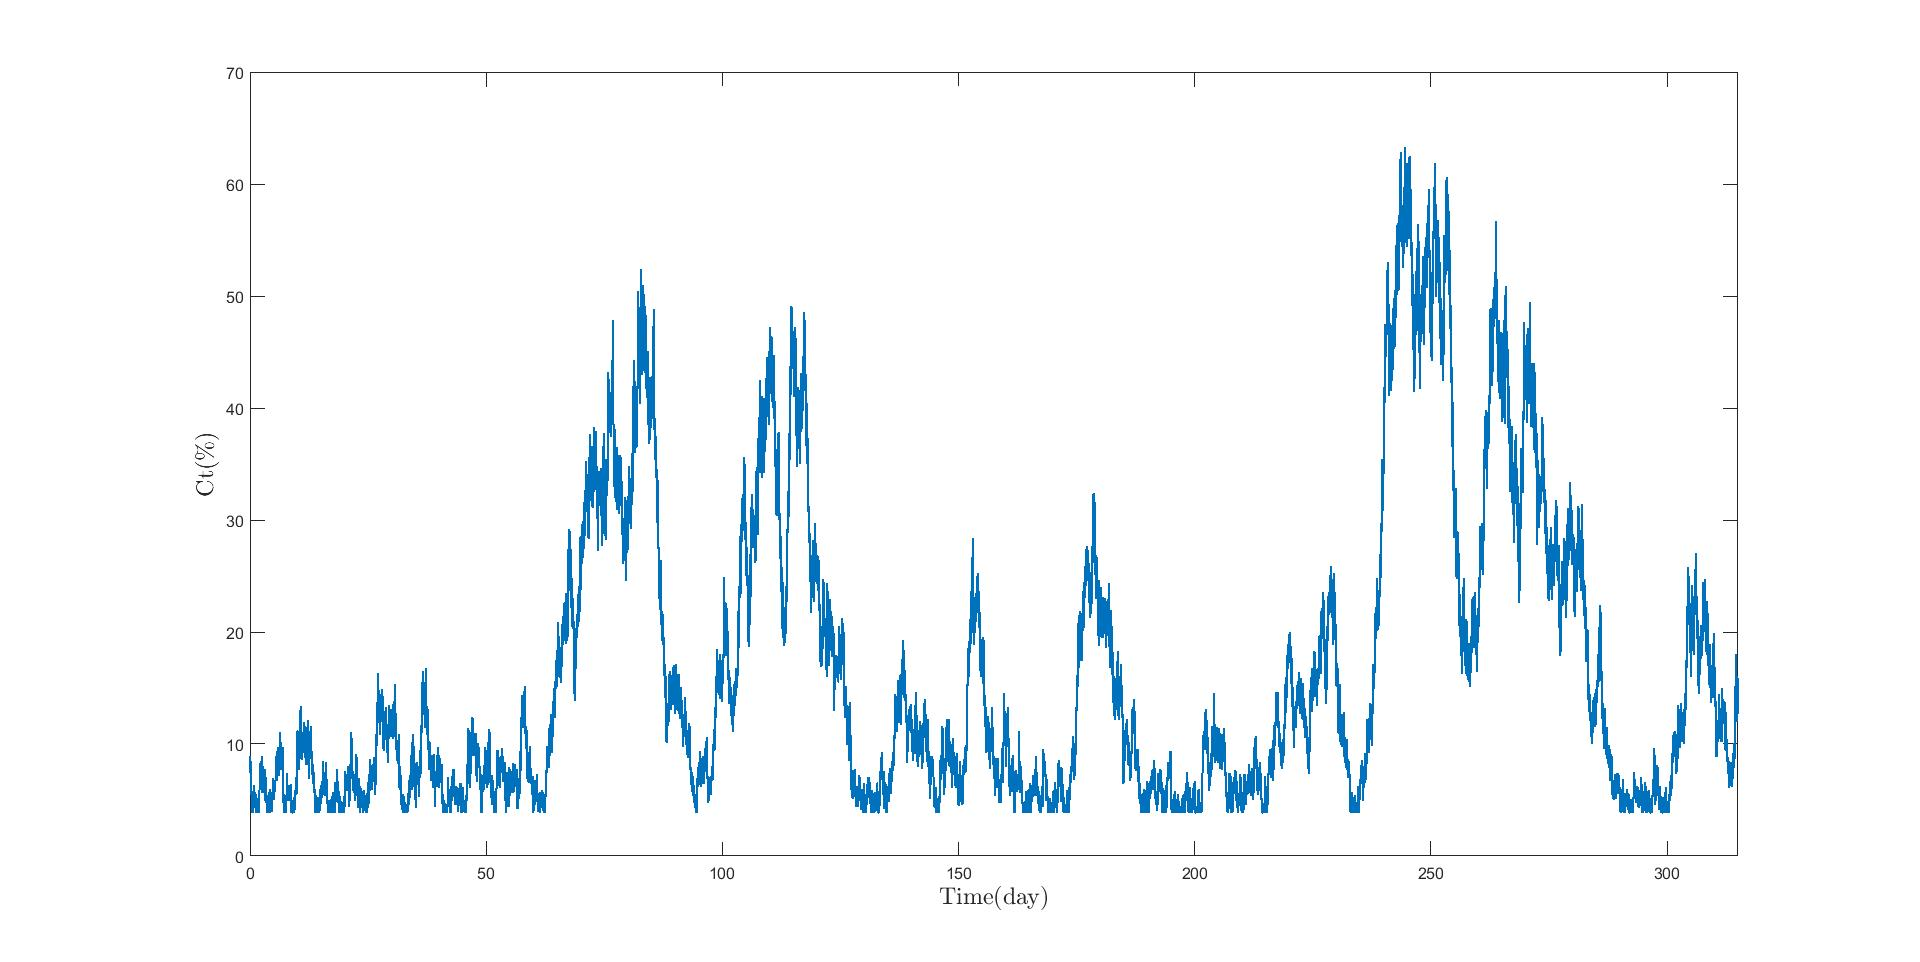
\includegraphics[width=15cm]{figures/p1_ex4_g1.jpg}
            \caption{Stochastic Volatility Ct with $\sigma_c=0.005$}
            \label{fig:4_g1}
            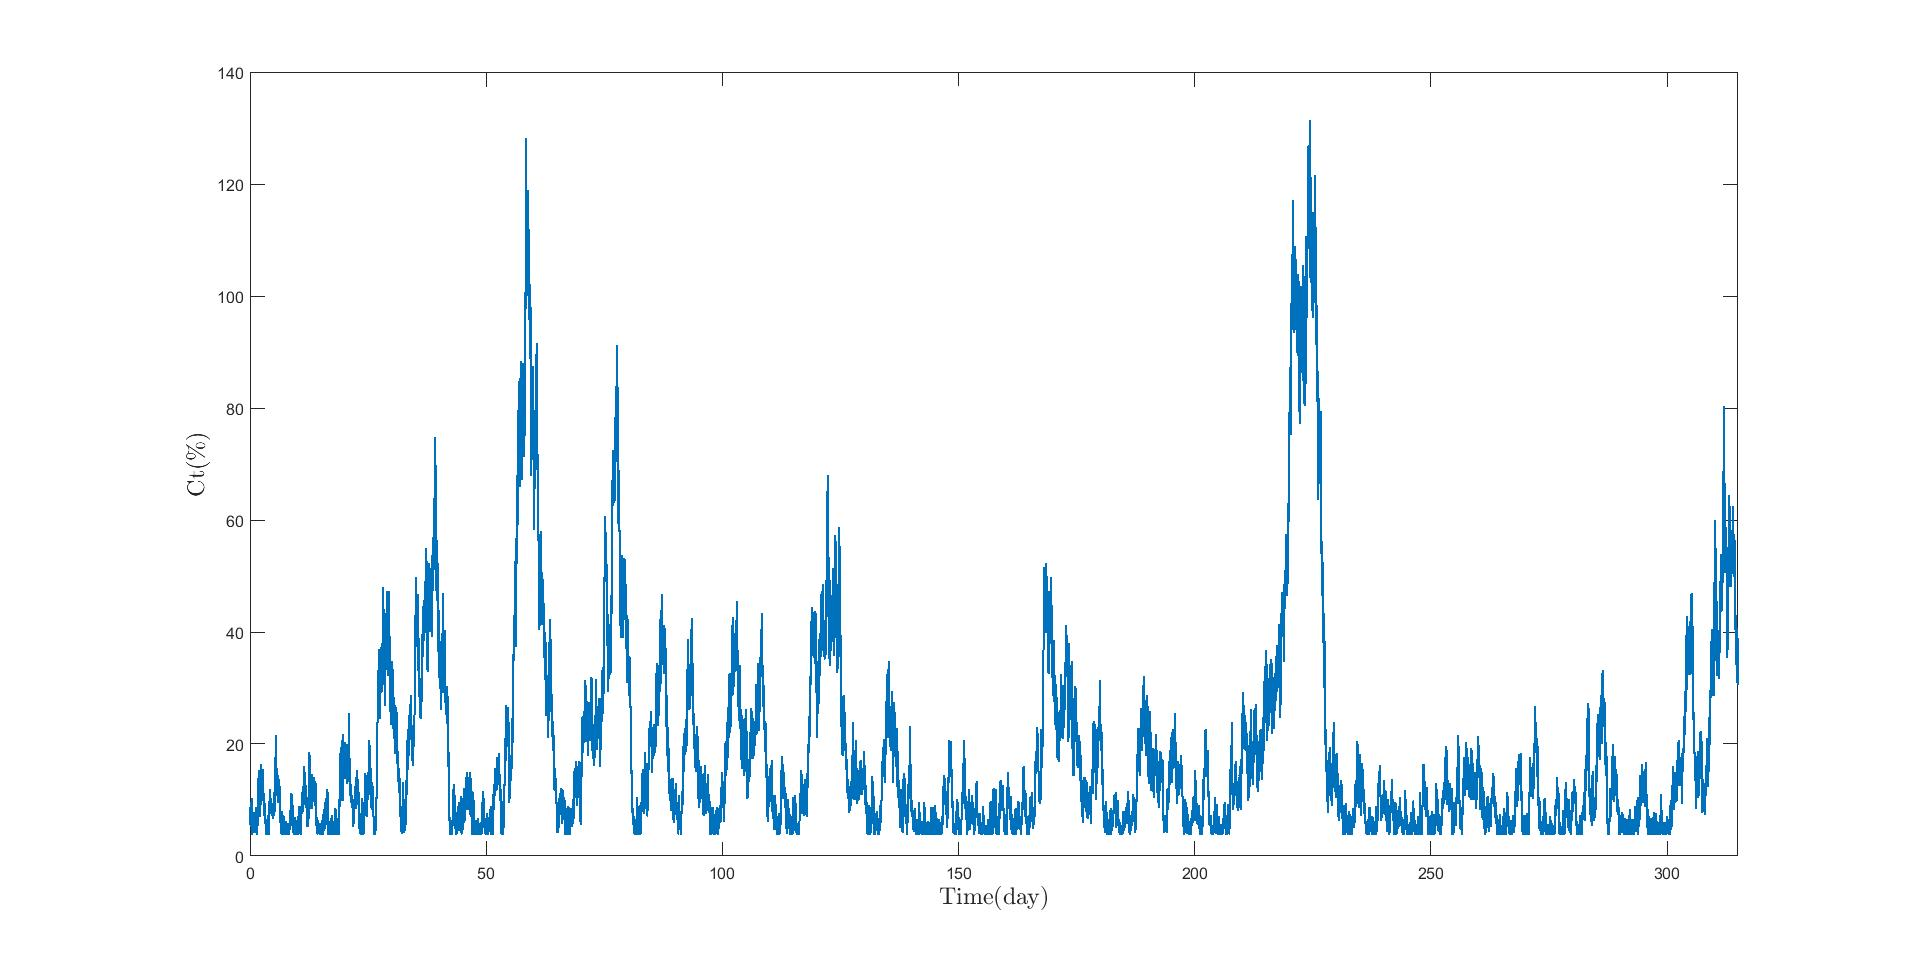
\includegraphics[width=15cm]{figures/p1_ex4_g2.jpg}
            \caption{Stochastic Volatility with $\sigma_c=0.01$}
            \label{fig:4_g2}
        \end{figure}
From the figure, we can find as the stochastic volatility with different volatility $\sigma$ increases from 0.005 to 0.01, the range of stochastic volatility Ct has doubled from $(\frac{\mu_c}{2},70)$ to  $(\frac{\mu_c}{2},140)$, the volatility of Ct increases.\\

The \textbf{MATLAB} code:
   \lstinputlisting{functions/JD_sv_ct.m}
    \lstinputlisting{functions/JD_sv_xt.m}
   \lstinputlisting{scripts/p1_ex4.m}
\end{enumerate}
\end{document}
